\documentclass[10pt]{article}

\usepackage[margin=1.2in]{geometry} % set margin size
\usepackage{fancyhdr}               % for headers/page numbers
\usepackage{booktabs}               % tabular settings
\usepackage{tabularx}               % better tables
\usepackage[bookmarks]{hyperref}    % additional PDF settings
\usepackage[parfill]{parskip}       % adjusting paragraph settings
\usepackage{todonotes}              % adding TODO notes
\usepackage{listings}               % source code listing
\usepackage{fontspec}               % for changing the font

% Style for source code listings
\lstset{basicstyle=\ttfamily\footnotesize, frame=single, tabsize=4, numbers=left}

% change the style for the header
\pagestyle{fancyplain}
\date{}
\setlength{\headheight}{18pt}

% use system font
\setmainfont{Droid Serif}
\setmonofont{Droid Sans Mono}

\def\doctitle{EE 119c Project Proposal}
\hypersetup{pdftitle={\doctitle}}

\title{Real-time Hand Tracking with Neural Nets on an FPGA}
\author{%
    \begin{tabular}{cc}
        Brian Kubisiak  & <bkubisia@caltech.edu> \\
        Quinn Osha      & <qosha@caltech.edu>
    \end{tabular}
}

\begin{document}

\lhead{\large{Brian Kubisiak, Quinn Osha}}
\chead{}
\rhead{\large{\today}}

\maketitle

\thispagestyle{empty}

\section{Functional Specification}
\label{sec:functional_specification}

For our project, we will be designing and implementing a system for tracking
a hand in real time from a camera input. The system will be implemented using a
Digilent Nexys 4 FPGA development board. It will take an input from a camera
connected to the USB port, analyze the data on the Artix 7 FPGA, and output each
from over the VGA port with a cursor overlay. The cursor overlay will indicate
where in the frame the hand is located. While the neural net is computing the
hand position, the frame will temporarily be stored in the board's memory---the
FPGA is too small to process an entire frame at once.

\subsection{Operation}
\label{sub:operation}

The FPGA design will consist of three distinct layers:
\begin{description}
    \item[Input Layer] For communicating with the USB camera, writing the frame
        to memory, and converting the frame into a format that the neural net
        can use.
    \item[Neural Network] For analyzing the camera data to determine where the
        hand is in the frame.
    \item[Output Layer] For reading the frame back from memory, overlaying a
        cursor on the hand position, and generating control signals to output
        the frame through a VGA port.
\end{description}

A top-level block diagram showing the layers and their connections is shown in
figure~(\ref{fig:top-level}). The Rx and Tx inputs come from the USB-UART
bridge. The Data, Address, Wr, and Rd signals go to the memory on the Digilent
board. Note that the Data and Address buses must be muxed before connecting to
the pins. The HSYNC, VSYNC, and Data outputs will go to the VGA port on the
board.

\begin{figure}[h]
    \centering
    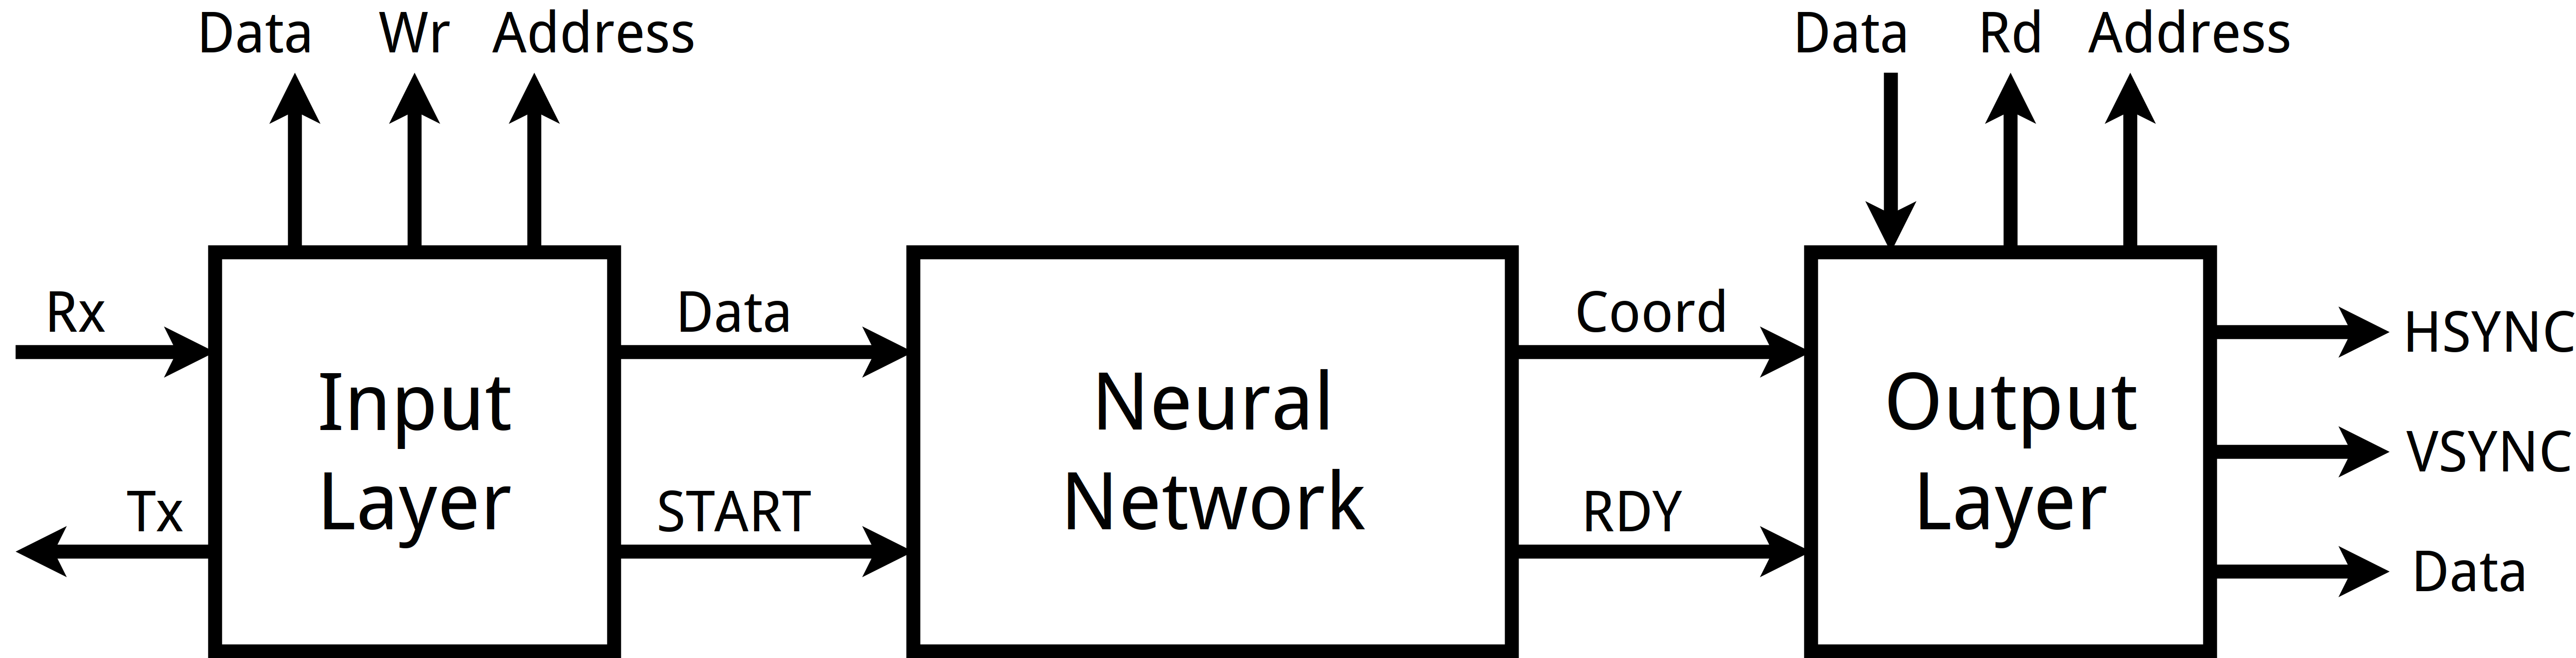
\includegraphics[width=0.8\linewidth]{diagrams/top-level.png}
    \caption{Top-level block diagram for the system.}
\label{fig:top-level}
\end{figure}

\subsubsection{Input Layer}
\label{ssub:input_layer}

The input layer is responsible for controlling the USB port, subsampling the
frame data, shifting the data into the neural net, and writing each frame into
memory. This process is shown in figure~(\ref{fig:input-layer}).

\begin{figure}[h]
    \centering
    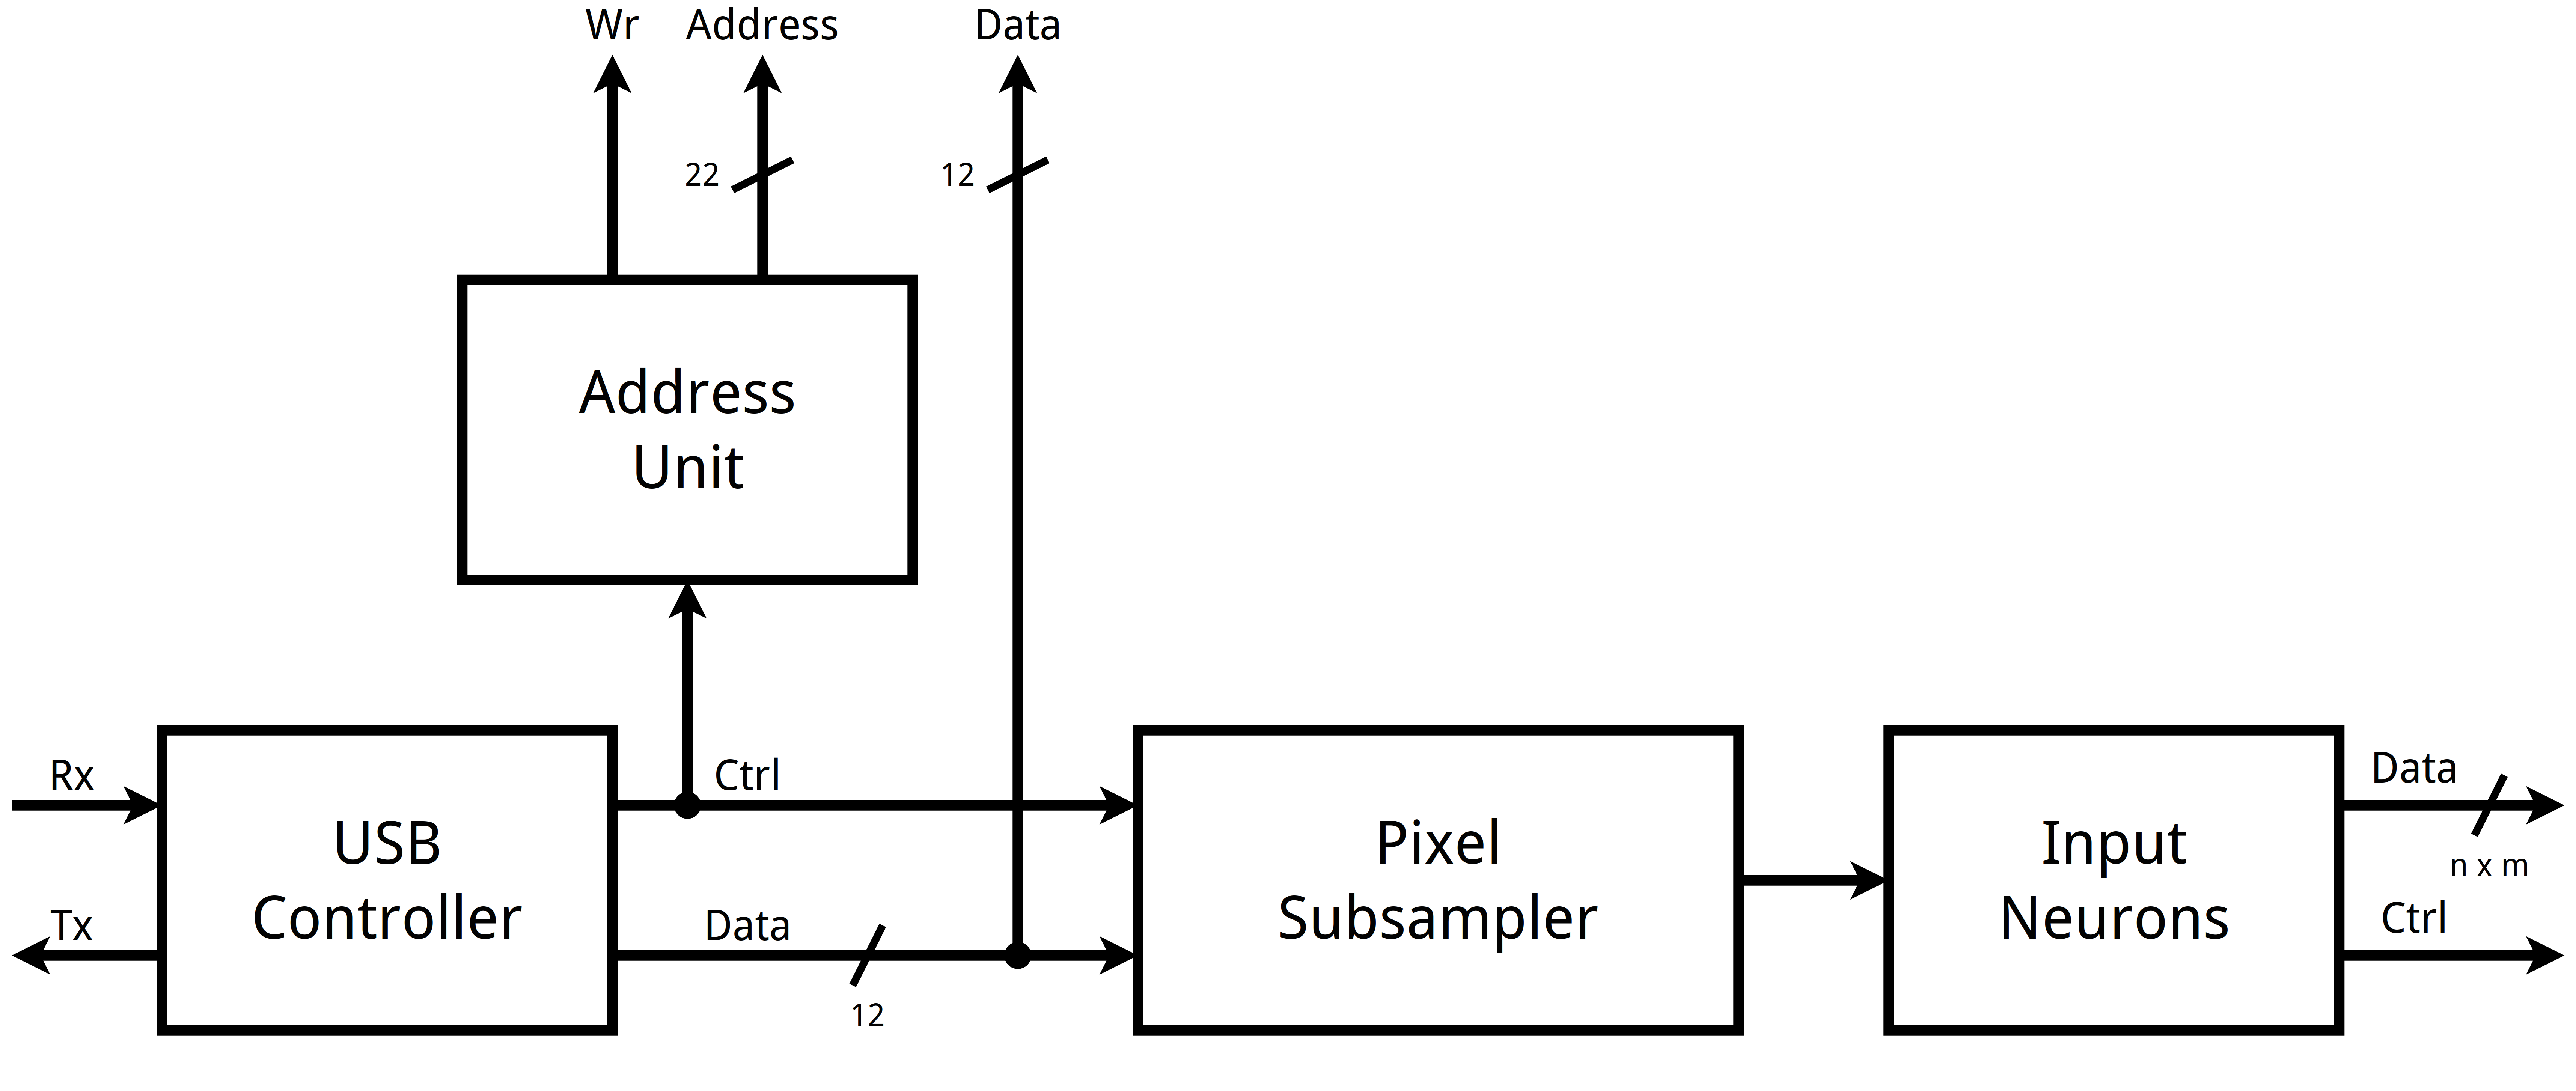
\includegraphics[width=0.8\linewidth]{diagrams/input-layer.png}
    \caption{Block diagram for the input layer.}
\label{fig:input-layer}
\end{figure}

The USB controller interfaces with the FT2232 USB-UART bridge on the Nexys 4
board through the Tx and Rx signals. The Tx signal is needed in order to give
commands to the camera over the USB port. The Rx line is responsible for reading
in the data.

Once the data is read in through the UART, it is parsed by a finite state
machine. This FSM will read the USB packets from the camera to extract the pixel
and frame data. It will condense each 24-bit pixel into 12 bits (the size needed
for the VGA) and output this data along with control signals for determining the
frame timing.

The address unit will take in the control signals from the USB controller and
use them to generate the proper addresses for the data. In order to improve
performance, the data will be written to memory in a format suitable for VGA
controller in the output layer. This address unit will take in the frame and
line data to ensure that the pixels are written to the proper addresses.
\todo{Figure out the memory layout that we need.}

Due to size limitations in the FPGA, the neural net cannot process the entire
frame. Pixels will be averaged togther in order to compress the data without
losing too much important information. \todo{Figure out how we want to
    subsample.}

The input neurons will take the subsampled data on a parallel bus and shift the
data through the input layer until the entire subsampled frame is loaded into
the neurons. These neurons will then output all $n \times m$ bits of frame data
to the neural net in parallel for processing. Control signals will tell the
neural net to start processing the frame.

\subsubsection{Neural Network}
\label{ssub:neural_network}

The neural network will take in the frame data and process it to determine the
coordinates of the hand in the frame. We will be using a multi-layer perceptron
(MLP) network to implement our design. The weights for each neuron will be
learned off chip, freeing up a lot of space for more neurons.

There will be an input neuron for each pixel in the subsampled frame. The input
neurons will be unique in that they will shift the data through the entire layer
in order to process the entire frame in parallel.

We will then have a single layer in the middle for the data processing. Each
neuron in this layer will have a single MAC unit and a sigmoid function. Since
the network will be trained off-chip, the weights will be pre-programmed into
the design. This will significantly reduce the size of the neurons.

The output layer will consist of only two neurons: one for computing the
x-coordinate of the hand, and another for computing the y-coordinate. The output
of the neural net will then just be a coordinate identifying where the hand is
in the frame.

\subsubsection{Output Layer}
\label{ssub:output_layer}

The output layer is responsible for converting the output of the neural net into
a group of pixel addresses, fetching the frame from memory, clearing the pixels
corresponding to the hand location, and outputting the frame using the VGA
protocol. A block diagram for this process is shown in
figure~(\ref{fig:output-layer}).

\begin{figure}[h]
    \centering
    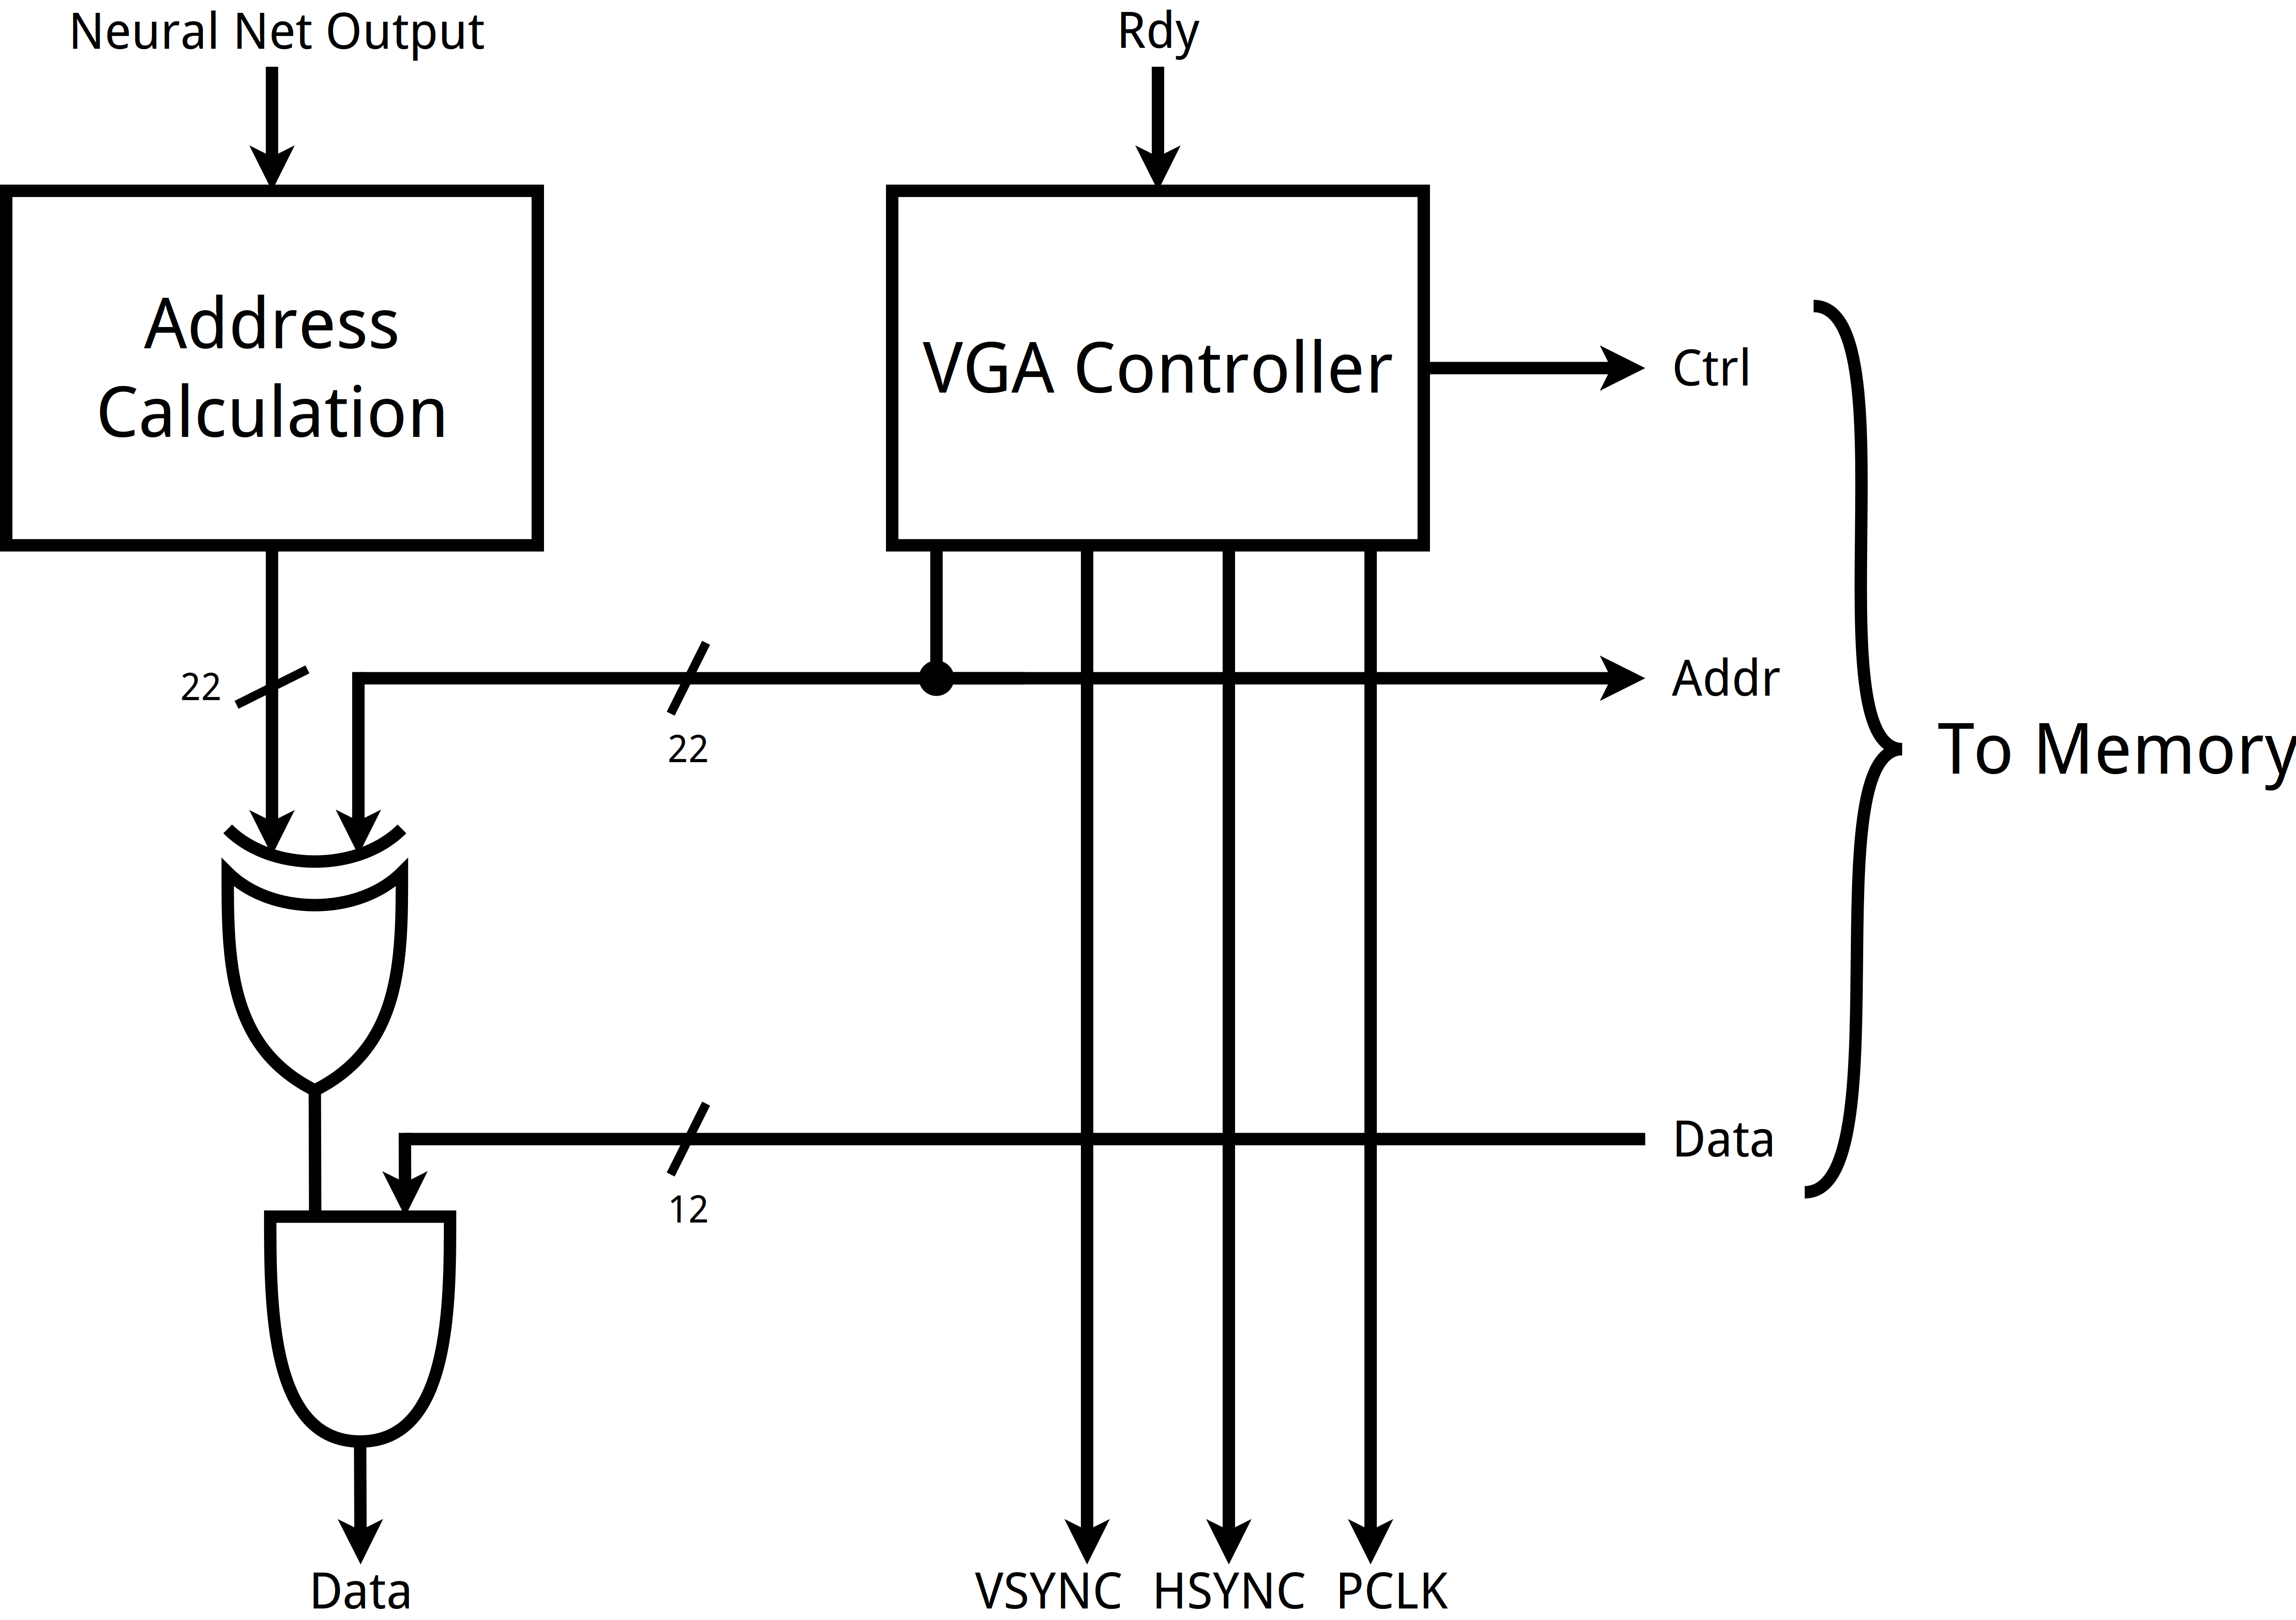
\includegraphics[width=0.6\linewidth]{diagrams/output-layer.png}
    \caption{Block diagram for the output layer.}
\label{fig:output-layer}
\end{figure}

The address calculation takes in the coordinates for the hand in the frame (from
the neural net) and converts them into a group of addresses. These addresses
correspond to the pixels in memory that will be blanked out for the cursor
overlay. These addresses are compared against the addresses output to the
memory, clearing the data output when they match.

The VGA controller is a finite state machine that begins running once it
receives the Rdy signal from the neural net. The controller will read the frame
from memory, one pixel at a time. It will also generate the proper line sync,
frame sync, and pixel clock signals to the VGA output. The data for the VGA
output will come directly from the data bus.

\subsection{Algorithms}
\label{sub:algorithms}

We will be using a neural network to identify where the hand is located in each
frame. The neural net will be organized as a multi-layer perceptron network. The
parameters for the neural network will be learned in advance on the computer,
then hard-coded into the FPGA neural net.

\subsection{Inputs}
\label{sub:inputs}

The input to this system will be video input through a USB controller. Each
frame that is input to the USB controller will be stored in an external memory
before being processed by the neural net.

\subsection{Outputs}
\label{sub:outputs}

The output from this system will be through a VGA controller. The VGA output
will be taken from an output frame buffer. The output frame will be generated
from the input frame with a cursor overlaid on the position of the hand
(identified by the neural net).

\section{Schedule}
\label{sec:schedule}

\setlength\extrarowheight{3pt}
\begin{tabularx}{\textwidth}{c X}
    Date & Tasks \\
    \midrule
    4/7--4/13 & Research current implementations of neural nets on FPGAs. Decide
    on video input and output devices (size and pixel depth). Write code for USB
    controller. \\
    4/14--4/20 & Write code for input data buffer and input data handling.
    Design---in a high-level-language---the desired neural net. \\
    4/21--4/27 & Test and configure the neural net on the computer. Write code
    for output data buffer and handling. \\
    4/28--5/4 & Begin coding the neural net on the FPGA\@. Write code for output
    display handling using VGA\@. \\
    5/5--5/11 & Finish coding the neural net. \\
    5/12--5/18 & Write code for the cursor video output. That is, given x and y
    coordinates, print the cursor at that point. \\
    5/19--5/25 & Write the top-level entity for the system, combining all the
    blocks. Train (unsupervised) the neural net. \\
    5/26--6/1 & Finish training the neural net. Fix any other bugs/issues. \\
    6/2--6/5 & Finish documentation and final touches.
\end{tabularx}

\section{Demonstration}
\label{sec:demonstration}

This system will be demonstrated by attaching a video camera to the USB input
and a monitor to the VGA output. Then, the system should detect a hand in the
input frame and output the frame to the monitor with a cursor overlaid on the
position of the hand.

\section{Source Code Listing}
\label{sec:source_code_listing}

Below is the VHDL source for our neural net and input/output layers. For a
high-level description of the design, see the functional specification.

\subsection{UART Receiver}
\label{sub:uart_receiver}

\lstinputlisting{src/uartrx.vhd}

\subsection{UART Transmitter}
\label{sub:uart_transmitter}

\lstinputlisting{src/uarttx.vhd}

\subsection{UART Receiver Testbench}
\label{sub:uart_receiver_testbench}

\lstinputlisting{src/uartrx-tb.vhd}

\subsection{UART Testbench}
\label{sub:uart_testbench}

\lstinputlisting{src/uart-tb.vhd}

\subsection{USB Video Decoder}
\label{sub:usb_video_decoder}

\lstinputlisting{src/usb_video_decoder.vhd}

\end{document}

